\documentclass{beamer}
%\usetheme{default}

\usetheme{JuanLesPins}
\usepackage{listings}
\usepackage{times}

%\usepackage{xkeyval}
\usefonttheme{structurebold}

\usepackage[english]{babel}
\usepackage{pgf}
%\usepackage{pgf,pgfarrows,pgfnodes,pgfautomata,pgfheaps,graphics}\usepackage{pgflibraryshapes}
%\usepackage{graphics}
\usepackage{epsfig}
\usepackage{amsmath,amssymb}
\usepackage[latin1]{inputenc}


%%%%%%%%%%%%%%CARDIS%%%%%%%%%%%%%%%%%%%%%%

\usepackage{tikz}
\usepackage{graphics}
\usepackage{pgflibraryshapes}

\usepackage{listings}

\lstset{escapeinside={(*@}{@*)}}
\lstset{commentstyle=\color{blue!50!black}\textit,tabsize=2,keywordstyle=\color{green!50!black}}
\lstset{backgroundcolor=\color{lightgray!50}}
%\lstset{frame=trbl,frameround=DDDD}
\lstset{numbers=left, numberstyle=\footnotesize}

\usepackage{multirow}
\newcommand{\benchname}[1]{\texttt{#1}}


\setbeamercovered{dynamic}%\beamertemplatenavigationsymbolsempty

\title[]{Java bytecode specification and verification}
\author[mariela.pavlova@sophia.inria.fr]{\textbf{Mariela Pavlova}}

\date[INRIA Sophia Antipolis ]{Institution: INRIA Sophia Antipolis\\
Supervisors: Gilles Barthe and Lilian Burdy}

\AtBeginSection[]{\frame{\frametitle{Outline}\tableofcontents[current]}}

\begin{document}

\begin{frame}
\titlepage
\end{frame}

%\newcommand{\stack}[1]{\mbox{\rm\textbf{st}}(#1)}% element on top stack 
%\newcommand{\counter}{\mbox{\rm\textbf{c}}}
%\newcommand{\locVar}[1]{\mbox{\rm{\textbf{reg}}}(#1) }





%%%%%%%%%%%%%%%%%%%%%%%%%%%%%%%%%%%%%%%%%%%%%%%%%%%%%%%%%%%%%%%%%%%%%%%%%%%%%%%%%%%%%%%%%%%%%%%%%%%%%%
%%%%%%%%%%%%%%%%%%%%%%%%%%%%%%%%%%%%%%%%BYTECODE LANGUAGE%%%%%%%%%%%%%%%%%%%%%%%%%%%%%%%%%%%%%%%%%%%%%%%%%%%
%%%%%%%%%%%%%%%%%%%%%%%%%%%%%%%%%%%%%%%%%%%%%%%%%%%%%%%%%%%%%%%%%%%%%%%%%%%%%%%%%%%%%%%%%%%%%%%%%%%%%%%%%%%%
 \newcommand{\bcIns}{\mbox{ \rm I} }
 \newcommand{\instrs}{\mbox{ \rm IS} }
 \newcommand{\ifCond}{ \instr{if\_cond } }
 \newcommand{\goto}{ \instr{goto } }
 \newcommand{\return}{ \instr{return } }
 \newcommand{\arithOp}{ \instr{arith\_op} }
 \newcommand{\load}{ \instr{load} }
 \newcommand{\store}{ \instr{store} }
 \newcommand{\push}{ \instr{push} }
 \newcommand{\pop}{\instr{pop}}
 \newcommand{\dup}{\instr{dup}}
 \newcommand{\iinc}{\instr{iinc}}
 \newcommand{\new}{\instr{new}}
 \newcommand{\newarray}{\instr{newarray}}
 \newcommand{\putfield}{\instr{putfield}} 
 \newcommand{\getfield}{\instr{getfield}}
 \newcommand{\arrstore}{\instr{type\_astore}} 
 \newcommand{\arrload}{\instr{type\_aload}}
 \newcommand{\arraylength}{\instr{arraylength}}
 \newcommand{\instanceof}{\instr{instanceof}} 
 \newcommand{\checkcast}{\instr{checkcast}} 
 \newcommand{\athrow}{\instr{athrow}}
 \newcommand{\invoke}{\instr{invoke}}
 \newcommand{\jsr}{\instr{jsr}}
 \newcommand{\ret}{\instr{ret}}
%%%%%%%%%%%%%%%%%%%%%%%%%%%%%%%%%%%%%%%%%%%%%%%%%%%%%%%%%%%%%%%%%%%%%%%%%%%%%%%%%%%%%%%%%%%%%%%%%%%%%%
%%%%%%%%%%%%%%%%%%%%%%%%%%%%%%%%%%%%%%%%BYTECODE LANGUAGE%%%%%%%%%%%%%%%%%%%%%%%%%%%%%%%%%%%%%%%%%%%%%%%%%%%
%%%%%%%%%%%%%%%%%%%%%%%%%%%%%%%%%%%%%%%%%%%%%%%%%%%%%%%%%%%%%%%%%%%%%%%%%%%%%%%%%%%%%%%%%%%%%%%%%%%%%%%%%%%%



\newcommand{\todo}[1]{\marginpar{\baselineskip0ex\rule{2,5cm}{0.5pt}\\[0ex]{\textsf{#1}}}}
\newcommand{\fig}[1]{ Fig.#1}
\newcommand{\jmlKey}[1]{\mbox{\rm\textbf{#1}}}% wrapping jml keywords
\newcommand{\java}[1]{\texttt{#1}}
\newcommand{\stack}[1]{\mbox{\rm\textbf{st}}(#1)}% element on top stack 
\newcommand{\stackOnly}{\mbox{\rm St}}
\newcommand{\stackOnlyParam}[1]{\mbox{\rm St}(#1)}
\newcommand{\newStack}{ \lbrack~\rbrack  } % empty stack
\newcommand{\update}[3]{ #1 [ \oplus {#2} \rightarrow {#3} ] }

\newcommand{\counter}{\mbox{\rm\textbf{cntr}} }
\newcommand{\counterOnly}{\mbox{\rm Cntr} }
\newcommand{\topStack}{\mbox{\rm cntr} }
\newcommand{\true}{\mbox{\rm\textbf{true}} } % true from the assertion language
\newcommand{\false}{\mbox{\rm\textbf{false}}} % false from the assertion language



\newcommand{\instr}[1]{\mbox{  \rm #1} }

%\newcommand{\loopStart}[1]{\textbf{loop\_start$\tt{_#1}$}}
%\newcommand{\loopEnd}[1]{\textbf{loop\_end$\tt{_#1}$}}
%\newcommand{\invariant}[1]{\it{I}_{\tt{#1}}}
%\newcommand{\boucle}[1]{\texttt{#1}}
%\newcommand{\loopModifies}[1]{\textbf{Modifies}(\texttt{#1}) }

\newcommand{\ins}[1]{instr_{#1}}
\newcommand{\insOnly}{\texttt{instr}}

% the grammar for the bytecode specification language
%\newcommand{\ClassSpec}{\rm{ClassSpec}}
%\newcommand{\ClassInv}{ClassInv}
%\newcommand{\ClassHistoryConstr}{ClassHistoryConstr}

%\newcommand{\MethodSpec}{\rm{MethodSpec}}


%\newcommand{\specCase}{\textrm{SpecCase}}
%\newcommand{\requires}{requires}
%\newcommand{\ensures}{ensures}
%\newcommand{\exsures}{exsures}
%\newcommand{\modifies}{modifies}

%\newcommand{\jmlStmt}[1]{\textrm{#1}}
%\newcommand{\specExpression}{\mathcal{E}^{spec}}

%\newcommand{\interMethodSpec}{\rm{InterMethodSpec}}
%\newcommand{\loopSpec}{\rm{loopSpec}}
%\newcommand{\assert}{\rm{assert}}

%\newcommand{\ArithExpr}{\texttt{ArithmeticExp} }

%\newcommand{\JMLExpr }{\texttt{JmlExp} }


\newcommand{\integer}{\texttt{int} }
\newcommand{\register}[1]{\mbox{\rm\textbf{reg}}(#1)}

\newcommand{\Mynull}{\jmlKey{null}}
\newcommand{\this}{\texttt{this}}
\newcommand{\fieldAccess}[2]{#1\mbox{\rm\textbf{.}}#2}
\newcommand{\arrayAccess}[2]{\mbox{\rm\textbf{arrayAccess}}( #1, #2) }  %{\mbox{\rm arrAccess}(#1, #2)}
\newcommand{\arrayAccessOnly}{\mbox{\rm arrAccess}}


%\newcommand{\loopInv}{loopInvariant}
%\newcommand{\loopMod}{loopModifies}

\newcommand{\result}{\jmlKey{$\backslash$result}}
%\newcommand{\old}[1]{\jmlKey{$\backslash$old(}#1\jmlKey{)}}
%\newcommand{\typeof}[1]{\jmlKey{$\backslash$typeof(}#1 \jmlKey{)}}
%\newcommand{\TYPE}{\jmlKey{TYPE} }
%\newcommand{\elemtype}[1]{ \jmlKey{$\backslash$elemtype(}#1\jmlKey{)} } 
%\newcommand{\excPost}{\psi^{exc}}

\newcommand{\Myspace}{\phantom{aaa}}
\newcommand{\predicate}{ \mathcal{P}} 
\newcommand{\Myfalse}{ \textit{false} }
\newcommand{\Mytrue}{ \textit{true} }



% abstractCtrlFlow.tex
\newcommand{\execRel}{\rightarrow} % the execution relation
\newcommand{\blockm}[1]{ \tt{b^{#1}} }
\newcommand{\blockSeq}[1]{ \tt{b_{seq}^{#1}} }
\newcommand{\pathm}[2]{\blockm{#1} \execRel^{*} \blockm{#2} }
\newcommand{\instrPost}[1]{ post(\instr{#1} )}
\newcommand{\invariant}{\textit{I}}




%from wp.tex
%\newcommand{\wpExeWithLoops}[1]{ \rm{Wp''}\rm{(#1)} }
%\newcommand{\wpExe}[1]{ \rm{Wp'}\rm{(#1)} }




\newcommand{\excPost}{\psi^{exc}}
\newcommand{\javaNull}{null}
\newcommand{\length}{\mbox{\rm arrLength}} % stands for array length


%%%%%%%%%%%%%%%%%%%%%%%%%%%%%%%%%%%%%%%%%%%%%%%%%%%%%%%%%%%%%%%%%%%%%%%%%%%%%%%%%%%%%%%%%%%%%%%%%%%%%%%%%%%%%%%%%%%%%%%%%%%%%%%%%%%%%%%%%%%%%%%%%%%%%%%%%%%%%%%%%%%%%%%%%%%%%%%%%%%%%%%%%%%%%%%%%%%%%%%%%%%%%%%%%%%%%%%%%%%%%%%%%%%%%%%%%%%%%%WP functions%%%%%%%%%%%%%%%%%%%%%%%%%%%%%%%%%%%%%%%%%%%%%%%%%%%%%%%%%%%%%%%%%%%%%%%%%%%%%%%%%%%%%%%%%%%%%%
%%%%%%%%%%%%%%%%%%%%%%%%%%%%%%%%%%%%%%%%%%%%%%%%%%%%%%%%%%%%%%%%%%%%%%%%%%%%%%%%%%%%%%%%%%%%%%%%%%%%%%%%%%%%%%%%%%%%%%%%%%%%%%%%%%%%%%%% 

\newcommand{\wpi}[3]{\mbox{\rm\textit{wp}}( #1, #2 , #3) }
\newcommand{\fwpi}{\mbox{\rm\textit{wp}}}
\newcommand{\inter}[2]{\mbox{ \rm \textit{inter}}(#1, #2, \methodd)} % predicate that holds between two bytecode blocks
\newcommand{\interOnly}{\mbox{ \rm \textit{inter}}} % the name of the function that calculates predicate that holds between two bytecode blocks
\newcommand{\objects}{\texttt{Objects}}

%%%%%%%%%%%%%%%%%%%%%%%%%%%%%%%%%%%%%%%%%%%%%%%%%%%%%%%%%%%%%%%%%%%%%%%%%%%%%%%%%%%%%%%%%%%%%%%%%%%%%%%%%%%%%%%%%%%%%%%%%%%%%%%%%%%%%%%%%%%%%%%%%%%%%%%%%%%%%%%%%%%%%%%%%%%%%%%%%%%%%%%%%%%%%%%%%%%%%%%%%%%%%%%%%%%%%%%%%%%%%%%%%%%%%%%%%%%%%%Heap%%%%%%%%%%%%%%%%%%%%%%%%%%%%%%%%%%%%%%%%%%%%%%%%%%%%%%%%%%%%%%%%%%%%%%%%%%%%%%%%%%%%%%%%%%%%%%%%%%%%%%%%%%%%%%%%%%%%%%%%%%%%%%%%%%%%%%%% 
%%%%%%%%%%%%%%%%%%%%%%%%%%%%%%%%%%%%%%%%%%%%%%%%%%%%%%%%%%%%%%%%%%%%%%%%%%%%%%%%%%%%%%%%%%%%%%%%%%%%%%%%%%%%%%%%%%%%%%%%%%%%%%%%%%%%%%%% 
\newcommand{\heap}{\mbox{\rm H}}
 \newcommand{\HeapSet}{\mbox{\rm \textsf{HeapType}}}
 \newcommand{\heapFields}{\mbox{\rm \textsf{Fld}}}
 \newcommand{\heapArrays}{\mbox{\rm \textsf{Arr}}}
 \newcommand{\heapLocs}{\mbox{\rm \textsf{Loc}}}
 \newcommand{\heapTypeOf}{\mbox{\rm \textsf{TypeOf }}}
 

\newcommand{\pc}{\mbox{\rm Pc}}
\newcommand{\field}[2]{\texttt{f}_{#2}^{#1}}
\newcommand{\Values}{\mbox{\rm\textit{Values}}}
\newcommand{\locVar}[1]{\mbox{\rm{\textbf{reg}}}(#1) }
\newcommand{\locVarOnly}{\mbox{\rm Reg}}


\newcommand{\AllRefs}{\mbox{\rm\textit{RefType}}} % the set all references  - reff \cup \reffArr  
\newcommand{\reff}{\mbox{\rm\textit{RefClType} }} % the type of simple reference
\newcommand{\reffArr}{\mbox{\rm\textit{RefArrType}}}
\newcommand{\Ref}[1]{\mbox{ \rm \texttt{ref}}_{#1}}
\newcommand{\reference}[1]{\mbox{ \rm \texttt{ref}}_{#1}}
\newcommand{\referenceOnly}{\mbox{ \rm \texttt{ref}} \ } 
\newcommand{\RefArr}[1]{\tt{refArr}_{#1} } % a reference to an array  ref_{type}^{length}
\newcommand{\substitution}[3]{#1 \lbrack #2 \leftarrow #3 \rbrack }
\newcommand{\subst}[2]{ \lbrack #1 \leftarrow #2 \rbrack }
\newcommand{\prevState}[1]{prev(#1)}
\newcommand{\nextState}[1]{next(#1)}


\newcommand{\RefValuesArr}{\mbox{\rm\textit{RefValArr}}}

\newcommand{\comment}[1]{ \{ \textit{ #1} \} }



\newcommand{\numConclusion}[1]{\textit{(#1)}}
\newcommand{\valueAtState}[2]{\it{val}_{#1}(#2)}

\newcommand{\stateTrans}{\hookrightarrow}
\newcommand{\stateTransTransClos}[1]{\longleftarrow_{#1}}

%%%%%%%%%%%%%%%%%%%%%%%%%%%%%%%%%%%%%%%%%%%%%%%%%%%%%%%%%%%%%%%%%%%%%%%%%%%%%%%%%%%%%%%%%%%%%%%%%%%%%%%%%%%%%
%%%%%%%%%%%%%%%%%%%%%%STATE CONFIGURATION%%%%%%%%%%%%%%%%%%%%%%%%%%%%%%%%%%%%%%%%%%%%%%%%%%%%%%%%%%%%%%%%%%%%
%%%%%%%%%%%%%%%%%%%%%%%%%%%%%%%%%%%%%%%%%%%%%%%%%%%%%%%%%%%%%%%%%%%%%%%%%%%%%%%%%%%%%%%%%%%%%%%%%%%%%%%%%%%%%
\newcommand{\configVar}{\mbox{\rm \textit{K}}}
\newcommand{\config}[5]{<{#1},{#2},{#3},{#4},{#5}>} % <\heap, \counter, \stackOnly, \locVarOnly , \pc>
\newcommand{\configFinalNorm}[3]{<{#1},{#2},{#3}>^{norm} }% the final configuration for a method's operational semantics   <\heap, RetValue> 
\newcommand{\configFinalExc}[3]{<{#1},{#2},{#3}>^{exc}}% the final configuration for a method's operational semantics   <\heap, excValue> 
\newcommand{\configFinal}[3]{<{#1},{#2},{#3}>^{final}} % config^final = config^exc + config^norm
\newcommand{\Final}{\mbox{\rm \textit{Final}}} % stands for result or the thrown exception
\newcommand{\SetConfigs}{\mbox{\rm \textit{K}}}
\newcommand{\SetConfigInterm}{\mbox{\rm \textit{K}}^{interm}}
\newcommand{\SetConfigFinal}{\mbox{\rm \textit{K}}^{final}}
\newcommand{\SetConfigFinalNorm}{\mbox{\rm \textit{K}}^{norm}}
\newcommand{\SetConfigFinalExc}{\mbox{\rm \textit{K}}^{exc}}

\newcommand{\termination}{\mbox{\rm End}}
\newcommand{\Res}{\mbox{\rm Res}}
\newcommand{\Exc}{\mbox{\rm Exc}} % the third component of a terminating configuration in  case of an exception

\newcommand{\eval}[2]{ #1 \vDash #2 } % \tau (expr )
\newcommand{\conf}[1]{\tt{<#1>}} % <\tau>

\newcommand{\bottom}{\bot}
%\newcommand{\pstate}[2]{<#1,#2> }
\newcommand{\RefValues}{\mbox{\rm\textit{RefVal}}}
\newcommand{\retValue}[1]{\textrm{returnVal}(#1)} % designates the result of the method
\newcommand{\objCl}[1]{\tt{Obj}_{#1}}% object representing a class instance 
\newcommand{\objArr}[2]{\tt{ObjArr}_{#1}^{#2}} % obj_{type}^{length} object representing an array instance
\newcommand{\modExp}{modExp}% stands for modfied locations by loops and methods


\newcommand{\method}{\mbox{ \rm m}~}
\newcommand{\excIndex}[2]{\mbox{ \rm \texttt{excIndex}}(#1,#2 ) }


%classFileExt.tex
\newcommand{\Myint}{\mbox{\rm\textbf{int}}}
%\newcommand{\intLiteral}{\texttt{int\_const} }
\newcommand{\predicates}{ \mathcal{R} }

\newtheorem{Formula}{Formulas}
\newtheorem{Predicate}{Predicates}

\newcommand{\formulaBc}{\mathcal{P}_{bml}}




%%%%%%%%%%%%%%%%%%Exception Types%%%%%%%%%%%%%%%%%%%%%%%%%5
\newcommand{\excType}{\mbox{\rm \textit{ExcType}}}
\newcommand{\NullPointerExc}{\mbox{ \rm \texttt{NullPntrExc}}}
\newcommand{\NegativeArraySizeExc}{\mbox{ \rm \texttt{NegArrSizeExc}}  }
\newcommand{\ArrIndexOutOfBoundExc}{\mbox{ \rm \texttt{ArrIndBndExc}} }
\newcommand{\ArithExc}{\mbox{ \rm \texttt{ArithExc}} }
\newcommand{\ClassCastExc}{\mbox{\rm \texttt{CastExc}}}
\newcommand{\Throwable}{\mbox{\rm \texttt{Throwable}}}
\newcommand{\ArrStoreExc}{\mbox{\rm \texttt{ArrStoreExc}} }

%%%%%%%%%%%%%%%%%%%%%%%%%%%%%%%%%%%%%%%%%%%%%%%%%%%%%%%%%%%%%%%%%%%%%%%%%%%%%%%%%%%%%%%%%%%%%%%%%%%%%%%%%%%%%
%%%%%%%%%%%%%%%%%%%%%%Class Fields Methods%%%%%%%%%%%%%%%%%%%%%%%%%%%%%%%%%%%%%%%%%%%%%%%%%%%%%%%%%%%%%%%%%%%%%%%%%%%%%%%%
%%%%%%%%%%%%%%%%%%%%%%%%%%%%%%%%%%%%%%%%%%%%%%%%%%%%%%%%%%%%%%%%%%%%%%%%%%%%%%%%%%%%%%%%%%%%%%%%%%%%%%%%%%%%%
 \newcommand{\class}{\mbox{ \rm Cl } }

 \newcommand{\FieldSet}{\mbox{\rm\textbf{Field}} } % the set of fields
 \newcommand{\FieldName}{\mbox{\rm\textbf{FieldName}}}
 \newcommand{\MethodSet}{\mbox{\rm\textbf{Method}} }
 \newcommand{\LoopSpecSet}{\mbox{\rm\textbf{LoopSpec}} }
 \newcommand{\MethodName}{\mbox{\rm\textbf{MethodName}} }
 \newcommand{\isField}[2]{\mbox{\rm\textsf{isfield}}(#1,#2)}
 \newcommand{\ClassSet}{\mbox{\rm\textbf{Class}}} % the  set of fields
 \newcommand{\ClassName}{\mbox{\rm\textbf{ClassName}}} % the set of fields
 
 \newcommand{\clazz}{\mbox{\rm \textit{C}}}
 \newcommand{\fieldd}{\mbox{\rm \textit{f}} }
 \newcommand{\methodd}{\mbox{\rm \texttt{m}}}

 %%%%%%%%%%%%%%%%%Class attributes %%%%%%%%%%%%%%%%%%%%%%%%%%%%%%%%%%%%%%%%%%%%%%%%%%%%%%%%%5
 \newcommand{\fields}{\mbox{\rm \textsf{fields}}}
 \newcommand{\methods}{\mbox{\rm \textsf{methods}}}
 \newcommand{\className}{\mbox{\rm \textsf{className}}}
 \newcommand{\superClass}{\mbox{\rm \textsf{superClass}}}
 \newcommand{\classCP}{\mbox{\rm \textsf{constantPool}}}
 %%%%%%%%%%%%%%%%%Field attributes%%%%%%%%%%%%%%%%%%%%%%%%%%%%%%%%%%%%%%%%%%%%%%%%%%%%%%%%%5
 \newcommand{\fieldName}{\mbox{\rm \textsf{Name}}}
 \newcommand{\fieldType}{\mbox{\rm \textsf{Type}}}
 \newcommand{\declaredIn}{\mbox{\rm \textsf{declaredIn}}}

 %%%%%%%%%%%%%%%%%Method attributes%%%%%%%%%%%%%%%%%%%%%%%%%%%%%%%%%%%%%%%%%%%%%%%%%%%%%%%%%5
 \newcommand{\methodName}{\mbox{\rm\textsf{Name}}}
 \newcommand{\retType}{\mbox{\rm\textsf{retType}}}
 \newcommand{\args}{\mbox{\rm\textsf{args}}}
 \newcommand{\numArgs}{\mbox{\rm\textsf{nArgs}}}
 \newcommand{\body}{\mbox{\rm\textsf{body}}}
 \newcommand{\entryPoint}{\mbox{\rm\textsf{entryPnt}}}
 \newcommand{\excHandlerTable}{\mbox{\rm\textsf{excHndlS}}}
 \newcommand{\exceptions}{\mbox{\rm\textsf{exceptions}}}
\newcommand{\methodLocVar}{\mbox{\rm\textsf{locVars}}}

\newcommand{\excPostSpec}{\mbox{\rm\textsf{excPost}}} % the postcondition that is specified in case the method ends with an exception exc 
\newcommand{\loopSpecTable}{\mbox{\rm\textsf{loopSpecS}}}
\newcommand{\normalPost}{\mbox{\rm\textsf{normalPost}}}
\newcommand{\pre}{\mbox{\rm\textsf{pre}}}
\newcommand{\modif}{\mbox{\rm\textsf{modif}}}

%%%%%%%%%%%%%%%%%Loop attributes%%%%%%%%%%%%%%%%%%%%%%%%%%%%%%%%%%%%%%%%%%%%%%%%%%%%%%%%%
\newcommand{\loopSpec}{\mbox{\rm\textit{loopSpec}}}



%%%%%%%%%%%%%%%%%Intra spec attributes%%%%%%%%%%%%%%%%%%%%%%%%%%%%%%%%%%%%%%%%%%%%%%%%%%%%%%%%%
\newcommand{\intraSpec}{\mbox{\rm\textit{assertion}}}
\newcommand{\atIndex}{\mbox{\rm\textbf{atIndex}}}


%%%%%%%%%%%%%%%%Exception handler%%%%%%%%%%%%%%%%%%%%%%%%%%%%%%%%%%%%%%%%%%%%%%%%%%%%%%%%%%%%%%%%%%%%
 \newcommand{\ExcHandler}{\mbox{\rm \textbf{ExcHandler}}}
 \newcommand{\excHH}{\mbox{\rm\textsf{excH}}} % stands for an instance of an ExceptioHandler type 
 \newcommand{\pcStart}{\mbox{\rm \textsf{startPc}}} 
 \newcommand{\pcEnd}{\mbox{\rm \textsf{endPc}}}
 \newcommand{\pcHandler}{\mbox{\rm \textsf{handlerPc}}}
  \newcommand{\exc}{\mbox{\rm \textsf{exc}}}



%%%%%%%%%%%%%%%%%%%%%%%%%%%%%%%%%%%%%
%%%%%%%%%%%%%%%%HEAP%%%%%%%%%%%%%%%%%%%%%
%%%%%%%%%%%%%%%%%%%%%%%%%%%%%%%%%%%%%
 \newcommand{\referenceDef}{\mbox{\rm ! }} % a function that decides if a reference exists and points to an existing object
 \newcommand{\referenceType}{\mbox{\rm isOfType} } % a function that decides that the reference is of some type 
 \newcommand{\JavaClass}{\mbox{\rm \textit{JClass}}} % the set of Java classes
 \newcommand{\JavaType}{\mbox{\rm\textit{JType}}} % the set of Java classes

 
 \newcommand{\isInList}[2]{\mbox{\rm \textit{inList}}(#1, #2)\ }
 \newcommand{\isInListOnly}{\mbox{\rm \textit{inList}}  }
 \newcommand{\addInList}[2]{\mbox{\rm cons}(#2, #1) } 
 \newcommand{\addInListOnly}{\mbox{\rm cons} } 
 \newcommand{\intersectOnly}{ \cap }
 \newcommand{\intersect}[2]{#1 \cap #2}
 \newcommand{\getFreshRef}[2]{\mbox{\rm getFreshRef}(#1,#2)}
 \newcommand{\getFreshRefOnly}{\mbox{\rm getFreshRef} \ }

 \newcommand{\newRef}[2]{\mbox{\rm newRef}(#1,#2 ) } % creates a new reference in the store
 \newcommand{\newRefOnly}{\mbox{\rm newRef}}
 \newcommand{\newArrRef}[3]{\mbox{\rm newArrRef}(#1,#2,#3) \ } % creates a new reference in the store
 \newcommand{\newArrRefOnly}{\mbox{\rm newArrRef}}

 \newcommand{\getLocations}[1]{\mbox{\rm getLoc}(#1) \ }
 \newcommand{\getLocationsOnly}{\mbox{\rm getLoc} \ } 
 \newcommand{\addNewLocation}[2]{\mbox{\rm allocator}(#1,#2) \ }
 \newcommand{\addNewLocationOnly}{\mbox{\rm allocator} \ }
 \newcommand{\defaultValue}[1]{\mbox{\rm\textsf{defVal}}(#1)} % default value for a type
 \newcommand{\defaultValueOnly}{\mbox{\rm \textit{defVal}}}
 \newcommand{\instanceFlds}[2]{\mbox{\rm \textit{instFlds}}(#1, #2)} % isInstField (field, class )
 \newcommand{\instanceFldsOnly}{\mbox{\rm \textit{instFlds}}}
 \newcommand{\InDom}[2]{\mbox{\rm\textit{inDom} } (#1,#2)} 
 \newcommand{\anyType}{\mbox{\rm \texttt{T}}} % represents any Java Type
 \newcommand{\Arrays}{\mbox{\rm ARR}} % an abstraction for all arrays in the heap

 %%%%%%%%%%%%%%%%%%% the state after  exception is thrown %%%%%%%%%%%%%%%%%%%%%%%%%%%%
 \newcommand{\getStateAfterExc}{\mbox{\rm \textit{getStateOnExc}\ }} 
 \newcommand{\findExcHandler}[3]{\mbox{\rm \textit{findExcHandler}}(#1,#2,#3)} % #1 = exception, #2 = pc , #3 = exception handler table 
 \newcommand{\findExcHandlerOnly}{\mbox{\rm\textit{findExcHandler}}\ } % #1 = exception, #2 = pc , #3 = exception handler table 



%%%%%%%%%%%%%%%%%%%%%%%%%%%%%%%%%%%%%%%%%%%%%%%%%%%%%%%%%%%%%%%%%%%%%%%%%%%%%%%%%%%%%%%%%%%
%%%%%%%%%%%%%%%%%%%%%%%%%%%%%%%%%Subtyping and types%%%%%%%%%%%%%%%%%%%%%%%%%%%%%%%%%%%%%%%%%%%%%%%%%%%%%%%%%%
%%%%%%%%%%%%%%%%%%%%%%%%%%%%%%%%%%%%%%%%%%%%%%%%%%%%%%%%%%%%%%%%%%%%%%%%%%%%%%%%%%%%%%%%%%% 
\newcommand{\subtypeOnly}{\mbox{\rm \textsf{subtype}}} 
\newcommand{\subtype}[2]{\mbox{\rm \textsf{subtype} }(#1,#2)}
 \newcommand{\Object}{\mbox{\rm \texttt{Object}} }


%%%%%%%%%%%%%%%%%%%%%%%%%%%%%%%%%%%%%%%%%%%%%%%%%%%%%%%%%%%%%%%%%%%%%%%%%%%%%%%%%%%%%%%%%%%
%%%%%%%%%%%%%%%%%%%%%%%%%%%%%%%%%constant pool%%%%%%%%%%%%%%%%%%%%%%%%%%%%%%%%%%%%%%%%%%%%%%%%%%%%%%%%%%
%%%%%%%%%%%%%%%%%%%%%%%%%%%%%%%%%%%%%%%%%%%%%%%%%%%%%%%%%%%%%%%%%%%%%%%%%%%%%%%%%%%%%%%%%%% 

\newcommand{\constantPool}{ \mbox{\rm\textbf{CP}}}
\newcommand{\localVariableTable}{\mbox{\rm\textbf{LV}}} 
\newcommand{\locVarEls}{\mbox{\rm\textbf{localVarTableElem}}}% an element of the local variable table
\newcommand{\lineNumberTable}{\mbox{\rm\textbf{LN}}} 
%%%%%%%%%%%%%%%%%%%%%%%%%%%%%%%%%%%%%%%%%%%%%%%%%%%%%%%%%%%%%%%%%%%%%%%%%%%%%%%%%%%%%%%%%%%
%%%%%%%%%%%%%%%%%%%%%%%%%%%%%%%%%BML%%%%%%%%%%%%%%%%%%%%%%%%%%%%%%%%%%%%%%%%%%%%%%%%%%%%%%%%%%
%%%%%%%%%%%%%%%%%%%%%%%%%%%%%%%%%%%%%%%%%%%%%%%%%%%%%%%%%%%%%%%%%%%%%%%%%%%%%%%%%%%%%%%%%%% 
\newcommand{\nonterminal}{ \mbox{\rm\textit{italics}} }
\newcommand{\terminal}{ \mbox{\rm\textbf{boldface}} }
\newcommand{\keyWord}{ \mbox{\rm\textsf{sans serif}} }

\newcommand{\expression}{\mbox{\rm\textit{E}}_{bml} }
\newcommand{\typeExp}{\mbox{\rm\textit{T}}_{bml}}
\newcommand{\expressions}{\mbox{\rm\textit{SpecExp}}_{bml}}

\newcommand{\Constants}{\mbox{\rm\textit{constants}}_{bml}}
\newcommand{\intLiteral}{\mbox{\rm\textit{intLiteral}}}
\newcommand{\signedInt}{\mbox{\rm\textit{signedIntLiteral}}}
\newcommand{\ident}{\mbox{\rm\textit{ident}}}
\newcommand{\idRef}{\mbox{\rm\textit{idRef}}}
\newcommand{\digit}{\mbox{\rm\textit{digit}}}
\newcommand{\digits}{\mbox{\rm\textit{digits}}}
\newcommand{\nonZeroDigit}{\mbox{\rm\textit{nonZerodigit}}}
\newcommand{\boundVar}{\mbox{\rm\textit{boundVar}}}
\newcommand{\bound}{\mbox{\rm\textbf{bv}}}
\newcommand{\unsignedInt}{\mbox{\rm\textit{unsignedInt}}}
\newcommand{\RefValuesSpec}{\mbox{\rm\textit{refVal}}}
\newcommand{\ClassSpec}{\mbox{\rm\textit{classSpec}}}
\newcommand{\MethodSpec}{\mbox{\rm\textit{methodSpec}}}
\newcommand{\specCase}{\mbox{\rm\textit{specCase}}}
\newcommand{\intraMethodSpec}{\mbox{\rm\textit{intraMethodSpec}}}
\newcommand{\modifiesLoc}{\mbox{\rm\textit{locations}}}
\newcommand{\specIndex}{ \mbox{\rm\textit{specIndex}}}
\newcommand{\op}{\mbox{\rm\textit{op}}}
\newcommand{\exsuresList }{\mbox{\rm\textit{exsuresList}}}

\newcommand{\mult}{\mbox{\rm\textbf{mult}}}
\newcommand{\divis}{\mbox{\rm\textbf{div}}}
\newcommand{\modulo}{\mbox{\rm\textbf{rem}}}
\newcommand{\plus}{\mbox{\rm\textbf{+}}}
\newcommand{\minus}{\mbox{\rm\textbf{-}}}

\newcommand{\bmlKeyWords}{ \mbox{\rm\textit{bmlKeyWords}} }

%%%%%%%%%%%%%%%%%%%%%%%%%%%%%%%%%%%%%%%%%%%%%%%%%%%%%%%%%%%%%%%%%% 
%%%%%%%%%%%%%%%%%%%%%%%%% method extension%%%%%%%%%%%%%%%%%%%%%%%%%%%%%%%
%%%%%%%%%%%%%%%%%%%%%%%%%%%%%%%%%%%%%%%%%%%%%%%%%%%%%%%%%%%%%%%%%%%%%%%%%%%% 
\newcommand{\posL}{\mbox{\rm\textsf{pos}}}
\newcommand{\invL}{\mbox{\rm\textsf{invariant}}}
\newcommand{\modifL}{\mbox{\rm\textsf{modif}}}
%%%%%%%%%%%%%%%%%%%%%%%%%%%%%%%%%%%%%%%%%%%%%%%%%%%%%%%%%%%%%%%%%% 
%%%%%%%%%%%%%%%%%%%%%%%%% BML keywords%%%%%%%%%%%%%%%%%%%%%%%%%%%%%%%
%%%%%%%%%%%%%%%%%%%%%%%%%%%%%%%%%%%%%%%%%%%%%%%%%%%%%%%%%%%%%%%%%%%%%%%%%%%% 
\newcommand{\ClassInv}{\mbox{\rm\textbf{ClassInv}}}
\newcommand{\ClassHistoryConstr}{\mbox{\rm\textbf{ClassHistoryConstr}}}
\newcommand{\declare}{\mbox{\rm \textbf{declare}} }
\newcommand{\ghost}{\mbox{\rm\textbf{ghost}}}
\newcommand{\locations}{\mbox{\textbf{locations}}}
\newcommand{\also}{ \mbox{\rm\textbf{also}}}
\newcommand{\requires}{\mbox{\rm\textbf{requires}}}
\newcommand{\ensures}{\mbox{\rm\textbf{ensures}}}
\newcommand{\exsures}{\mbox{\rm\textbf{exsures}}}
\newcommand{\modifies}{\mbox{\rm\textbf{modifies}}}
\newcommand{\assert}{\mbox{\rm \textbf{assert}}}
\newcommand{\set}{\rm\textbf{set}}
\newcommand{\loopInv}{\mbox{\rm\textbf{loopInv}}}
\newcommand{\loopMod}{\mbox{\rm\textbf{loopModif}}}

\newcommand{\loopDecreases}{\mbox{\rm\textbf{loopDecreases}}}
%%%%%%%%%%%%%%%%%%%%%%%%%%%%%%%%%%%%%%%%%%%%%%%%%%%%%%%%%%%%%%%%%% 
%%%%%%%%%%%%%%%%%%%%%%%%%%%%%%%%%%%%%%%%%%%%%%%%%%%%%%%%%%%%%%%%%% 

\newcommand{\jmlStmt}[1]{\textrm{#1}}
\newcommand{\specExpression}{\mathcal{E}^{spec}}

\newcommand{\EXC}{ \mbox{$\backslash$\rm\textbf{EXC}}} % SPEC the spec variable used in exceptional postconditions to denote the thrown exception object




\newcommand{\ArithExpr}{\texttt{ArithmeticExpr} }

\newcommand{\JMLExpr }{\texttt{JmlExp} }

\newcommand{\everything}{\mbox{\rm \textbf{everything}}}
\newcommand{\nothing}{\mbox{\rm  \textbf{nothing}}}
\newcommand{\arrayAccessMod}[2]{\mbox{\rm\textit{arrayModAt}}(#1,#2)}

\newcommand{\all}{ \mbox{\rm all}}




%\newcommand{\result}{\jmlKey{$\backslash$result}}
\newcommand{\old}[1]{\jmlKey{$\backslash$old(}#1\jmlKey{)}}
\newcommand{\typeof}[1]{\jmlKey{$\backslash$typeof(}#1 \jmlKey{)}}
\newcommand{\subtypeSpec}{<:}
\newcommand{\type}[1]{\jmlKey{$\backslash$type(}#1 \jmlKey{)}}
\newcommand{\TYPE}{\jmlKey{$\backslash$TYPE} }
\newcommand{\elemtype}[1]{ \jmlKey{$\backslash$elemtype(}#1\jmlKey{)} } 
%\newcommand{\excPost}{\psi^{exc}}





%%%%%%%%%%%%%%%%%%%%%%%%%%%%%%%%%%%%%%%%%%%%%%%%%%%%%%%%%%%%%%%%%%%%%%%%%%%%%%%%%%%%%%%%%%%%%%%%%%%%%%%%%
%%%%%%%%%%%%%%%%%%%%%%%%%%%%%%%%%%%%5interpetation%%%%%%%%%%%%%%%%%%%%%%%%%%%%%%%%%%%%%%%%%%%%%%%%%%%%%%%%%%%%%%
%%%%%%%%%%%%%%%%%%%%%%%%%%%%%%%%%%%%%%%%%%%%%%%%%%%%%%%%%%%%%%%%%%%%%%%%%%%%%%%%%%%%%%%%%%%%%%%%%%%%%%%%%
\newcommand{\evalExp}[2]{\mbox{ \rm \textit{eval}}( #1,#2 )} % evaluation of an expression #1 in  a state configuration #2
\newcommand{\evalRel}[1]{\mbox{ \rm \textit{rel}}( #1 )} % evaluation of an expression #1 in  a state configuration #2

\newcommand{\interp}[2]{#2 \vDash #1} % interpretation of a predicate  #1 in  a state configuration #2
\newcommand{\interpTwoLines}[2]{ \begin{array}{l} #2  \vDash \\ 
				         #1 
				  \end{array}}

%%%%%%%%%%%%%%%%%%%%%%%%%wpbc%%%%%%%%%%%%%%%%%%%%%%%%%%%%%%%%%%%
\newcommand{\modifLoop}{\mbox{\rm \textit{modifLoop}}}


%%%%%%%%%%%%%%%%%%%%%%%%%%%%%%%%%%%%%%%%%%%%%%%%%%%%%%%%%%%%%%%%%%%%%%%%%%%%%%%%%%%%%%%%%%%%%%%%%%%%%%%%%
%%%%%%%%%%%%%%%%%%%%%%%%%%%%%%%%%%%% local variable table %%%%%%%%%%%%%%%%%%%%%%%%%%%%%%%%%%%%%%%%%%%%%%%%%%%%%%%%%%%%%%
%%%%%%%%%%%%%%%%%%%%%%%%%%%%%%%%%%%%%%%%%%%%%%%%%%%%%%%%%%%%%%%%%%%%%%%%%%%%%%%%%%%%%%%%%%%%%%%%%%%%%%%%%
\newcommand{\nameInd}{\mbox{\rm\textsf{nameIndex}}}
\newcommand{\attLen}{\mbox{\rm\textsf{attrLen}}}
\newcommand{\lvLength}{\mbox{\rm\textsf{lvLength}}}
\newcommand{\lvTab}{\mbox{\rm\textsf{lvTable}}}
%%%%%%%%%%%%%%%%%%%%%%%%%%%%%%%%%%%%%%%%%%%%%%%%%%%%%%%%%%%%%%%%%%%%%%%%%%%%%%%%%%%%%%%%%%%%%%%%%%%%%%%%%
%%%%%%%%%%%%%%%%%%%%%%%%%%%%%%%%%%%% element in the array of local variable table %%%%%%%%%%%%%%%%%%%%%%%%%%%%%%%%%%%%%%%%%%%%%%%%%%%%%%%%%%%%%%
%%%%%%%%%%%%%%%%%%%%%%%%%%%%%%%%%%%%%%%%%%%%%%%%%%%%%%%%%%%%%%%%%%%%%%%%%%%%%%%%%%%%%%%%%%%%%%%%%%%%%%%%%
\newcommand{\lvElStart}{\mbox{\rm\textsf{startPc}}}
\newcommand{\lvElLen}{\mbox{\rm\textsf{length}}}
\newcommand{\descrInd}{\mbox{\rm\textsf{descrInd}}}
\newcommand{\lvElInd}{\mbox{\rm\textsf{index}}}

%%%%%%%%%%%%%%%%%%%%%%%%%%%%%%%%%%%%%%%%%%%%%%%%%%%%%%%%%%%%%%%%%%%%%%%%%%%%%%%%%%%%%%%%%%%%%%%%%%%%%%%%%
%%%%%%%%%%%%%%%%%%%%%%%%%%%%%%%%%%%% the deep expression language %%%%%%%%%%%%%%%%%%%%%%%%%%%%%%%%%%%%%%%%%%%%%%%%%%%%%%%%%%%%%%
%%%%%%%%%%%%%%%%%%%%%%%%%%%%%%%%%%%%%%%%%%%%%%%%%%%%%%%%%%%%%%%%%%%%%%%%%%%%%%%%%%%%%%%%%%%%%%%%%%%%%%%%%
\newcommand{\exprWp}{\mbox{\rm\textit{E}}}
\newcommand{\predWp}{\mbox{\rm\textit{P}}}
\newcommand{\constantsWp}{\mbox{\rm\textit{constants}}}
\newcommand{\expressionsWp}{\mbox{\rm\textit{Expr}}}
\newcommand{\typeExpWp}{\mbox{\rm\textit{T}}}
\newcommand{\refWp}{\mbox{\rm\textbf{ref}}}
\newcommand{\ConstantsWp}{\mbox{\rm\textit{constants}}}


\newcommand{\wpi}{\mbox{\rm\textit{wp}}}%\xspace}
\newcommand{\Pred}{\mbox{\rm\texttt{Pred}}}
%\newcommand{\ins} {\mbox{\rm\texttt{Ins}}}
\newcommand{\program}{\mbox{\rm\texttt{P}}}%\xspace}
\newcommand{\Method}{\mbox{\rm\texttt{Method}}}% method type \xspace}
\newcommand{\methodd}{\mbox{\rm\textit{m}}}

%\newcommand{\subst}[2]{[ #1 \backslash #2]}
%\newcommand{\requires}{\texttt{requires}}
%\newcommand{\ensures}{\texttt{ensures}}
%\newcommand{\annotation}{BML}
%\newcommand{\exsures}[1]{ \texttt{exsures} (#1)}
%\newcommand{\invariant}{ \texttt{invariant}}
%\newcommand{\variant}{ \texttt{variant}}
%\newcommand{\ghost}{ \texttt{Model}}
%\newcommand{\declare}{ \texttt{declare}}
%\newcommand{\assert}{ \texttt{assert}}
%\newcommand{\modifies}{ \texttt{modifies}}
%\newcommand{\ghostSet}{ \texttt{set}}
%\newcommand{\expression}{\mathcal{E}}
%\newcommand{\predicate}{\mathcal{P}}
% \input mydef.tex   



\section{Context}
\begin{frame}[shrink]
\frametitle{Mobile code}
Welcome to Imserba\bigskip\\

The best mobile phones portal and community in the world
Mobile phones Portal and Community\bigskip\\  

Imserba brings you the latest mobile phones related \\
news, informations, stuffs you need for your phones. \\
No matter which phone you are using: Nokia, Sony\\
erricson, Siemens, Samsung, Motorola or anything\\ 
else, here you can find our best collection of ring- \\
tones, cell phone games, themes, screensavers,\\
backgrounds
\begin{center}
\pgfimage[width=4cm]{figs/beestje}
\end{center}    
\alert{Are you sure that you can trust these applications?} 
\end{frame}


% \begin{frame}[shrink]\frametitle{Mobile code}
%   \begin{definition}{Mobile code}
%    small pieces of software automatically downloaded into
%    the user's workstation and executed without the user's initiation or knowledge.
%   \end{definition}
% \begin{center}
% % 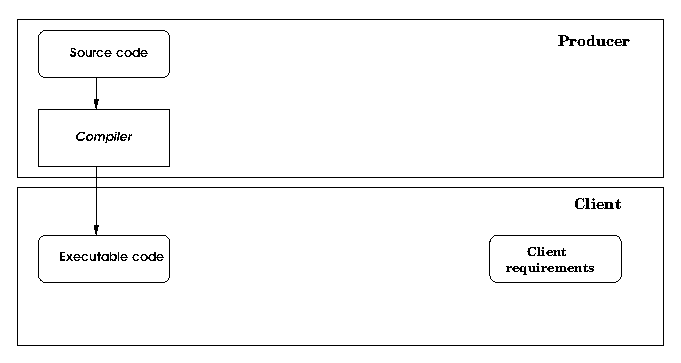
\epsfig{file=figs/mobileCode.eps}
% \end{center}
%  \end{frame}

% security trusted personal devices 
% are used for security sensitive applications, they manage confidential data
% and rely on limitted resources
\begin{frame}
\frametitle{Security and trusted personal devices}
\begin{itemize}
\item Trusted personal devices: phones, smart cards, pda's, set
top boxes, \dots
\item Used for security-sensitive applications
\item Network connected
%\item Support for complex applications (contain a full JVM)
%\item Shift from hardware attacks to logical attacks
\end{itemize}
\end{frame}


\begin{frame}\frametitle{Mobile code and Java}
 % the de facto language for web applications , mobile phones, what ever smart cards
The de facto language for web applications:
 \begin{itemize}
  \item platform independent execution framework
  \item  With the JVM available in most popular browsers, the concept of mobile code was born
  \item widely used in   smart card applications
 \end{itemize}

Security guarantees: 
\begin{itemize}
    \item type safety
     \item sandbox mechanism
\end{itemize}

But malicious code may also use 
\begin{itemize}
     %\item logical attacks
     \item resource attacks
       \item information leaks
	 \item or does not respect the internal invariants of the host system
\end{itemize}
\end{frame}

\begin{frame}\frametitle{Guaranteeing security }
\begin{itemize}
     \item Digital signatures - trusting the signer does not mean that there are no errors or bugs in the code
     \item Runtime checking -  expensive, incurs runtime overhead
     \item Formal verification - relies on rigorous modelisation of the programming language and its semantics.
                          Does not have runtime cost. Provides means to guarantee that the unknown code respects 
			  the client requirements
 \end{itemize}
\end{frame}

\begin{frame}[shrink,fragile]\frametitle{Formal verification}
  \begin{itemize}
    \item Specification language 
        % \begin{itemize}
	%    \item formalism for expressing program properties, e.g. 
	%      what are the desirable 
	%%      conditions that  must hold over the program input and output
	%  \end{itemize}
    \item Generation of conditions which express program correctness
         w.r.t. the specification
       %\begin{itemize}
	%  \item directly on the operational semantics, requires 
		%    intensive user interaction
	 % \item Hoare logic, provides inference rules which allow for 
	  %   automation, still need user interaction
	 % \item verification condition generators, automatic generation
	  %   of formulas, which guarantee program correctness
      % \end{itemize}
    \item Proving the condition that express that the program 
          is correct w.r.t. the specification
       % \begin{itemize}
	%    \item automatic decision procedures
%	    \item interactive theorem prover
%	\end{itemize}
  \end{itemize}

\begin{center}
\pgfimage{figs/sourceVerification}
\end{center}
\end{frame}


\begin{frame}\frametitle{The formal specification language JML}
 JML stands for  Java Modeling Language and is the de facto specification of JML
  \begin{itemize}
     \item Contract based approach
             % \begin{itemize}
	     %    \item preconditions
	%	 \item postconditions
	 %    \end{itemize}
     
       \item Method annotations
	 %  \begin{itemize}
	 %         \item loop invariants 
	 %	   \item assertions at particular program points
	  %   \end{itemize}
 %
	          \item Special specification constructs  
	 %  \begin{itemize}
	   %       \item keywords \lstinline!\TYPE!, \lstinline!\result!
	 %	 \item operators   \lstinline!\old(e)!, \lstinline!\typeof(e)!
	 %	 \item specification variables   
	  %   \end{itemize}
         \item \ldots

  \end{itemize}
\end{frame}

\begin{frame}[fragile,shrink]\frametitle{JML.Example}
  \begin{lstlisting}[language=java]
//@ requires k >= 0 ;
//@ ensures \result == k*(k+1)/2;
public int sum (int k) {
  int sum = 0;		
  //@loop_modifies sum,i;
  //@loop_invariant i >= 0 && i<=k && 
  //@               sum == i*(i+1)/2;
  for  (int i = 0; i < k; i++ ) {
    sum = sum + i;
  } 	
  return sum;
}
\end{lstlisting} 
\end{frame}



 \begin{frame}[shrink]\frametitle{Program calculi. Weakest precondition  predicate transformers}
   \begin{definition}[Definition of \wpName{} ]

   $$ \begin{array}{l} 
       \wpName : \stmt \cup \expressionSrc \rightarrow \Pred   \rightarrow \Pred   \\
       \wpSrcStmt{ \var = \expressionSrc}{\normalPostSrc } =  \wpSrcExpr{\expressionSrc}{\normalPostSrc \subst{\var}{v} }{v} \\
    \end{array}
$$
      \end{definition} 

  \begin{definition}[Method respects its specification]
     If a method \methodd{} with precondition  \methodd.$Pre$
        and postcondition \methodd.$Post$ starts execution in state $s_0$ , and terminates execution in $s_1$, i.e.  \ $\methodd: \  s_0  \stateTransTerm s_1 $ 
          and $s_0 \vDash \methodd.Pre $ holds    
         then $s_1 \vDash \methodd.Post$ holds
       \end{definition}
 %\end{frame}

 % \begin{frame}\frametitle{Program calculi. Weakest precondition  predicate transformers}
     \begin{theorem}[Soundness of  \wpName{}]
        If a method \methodd{} with precondition  \methodd.$Pre$
        and postcondition \methodd.$Post$ is such that 
        the verification conditions are valid formulas 
$ \vDash \methodd.Pre \Rightarrow \wpSrcStmt{\methodd.body}{\methodd.Post } $ 
        then \methodd{} respects its specification in the sense of the upper definition
       \end{theorem}    
   
 \end{frame}


\begin{frame}\frametitle{Java program verification tools}

The list of Java program verification tools is long 
\begin{itemize}
   \item  The Loop tool
     \item ESC/java
       \item Krakatoa
	 \item Jive
	  % \item the Key project
	     \item JACK 
	       \item \ldots
\end{itemize}
\end{frame}



% \begin{frame}\frametitle{History of JACK}
%\begin{itemize}
%\item Development started at Gemplus (Jan 2002 to April 2003)\\
%Objective: Give developers tools that help them to provide and be
%accountable for quality of their code
%\begin{itemize}
%\item Conform to specification requirements
%\item Well-documented
%\item Without bugs
%\end{itemize}
%\item Transfered to INRIA (September 2003)
%\end{itemize}
%\end{frame}



\begin{frame}\frametitle{Features of JACK}
\begin{itemize}
\item Tight integration with IDE Eclipse
\item JML used as annotation language
\item Support for Simplify (automatic) and Coq (interactive) prover
\item User friendly interface
\end{itemize}
\end{frame}


\begin{frame}[shrink,fragile]\frametitle{Developing an application in Eclipse}
\vspace*{-1.5em}
\pgfimage[height=\textheight]{figs/screen1}
\end{frame}

% source not sufficient
\begin{frame}\frametitle{However...}
  Source verification not always suitable
   \begin{itemize}
     \item In mobile code  scenarios, the client receives only the
           executable code    
    %\item And even if the executable is accompanied with the source code, 
     %  the client probably does not trust the compiler
     %\item software audit which does not trust the compiler
     \item Need for techniques which allow to reason on low level languages   
     \item George Necula and Peter Lee propose the Proof Carrying Code (PCC) architecture
       which allows establishing trust in the unknown executable code
   \end{itemize}  
\end{frame}

\begin{frame}
\frametitle{PCC architecture}
\begin{center}
\pgfimage[height=\textheight]{figs/PCC}
\end{center}
\end{frame}

\begin{frame}
\frametitle{Limitation of traditional PCC}
\begin{itemize}
 \item Suitable for properties like
       well typedness or safe memory read write access 
 \item However,% with the development of the network software technologies, 
       the security requirements also become more complex and 
       may go beyond safety properties 
            
  \item  Need to transfer the verification and expressive power of source verification techniques
        to executable code  in order to check the mobile code against complex functional policies 

\end{itemize}
\end{frame}


\begin{frame}\frametitle{PCC architecture for complex policies}
   \begin{center}
       \pgfimage[height=\textheight]{figs/PPO}
   \end{center}
\end{frame}
%%%%%%%%%%%%%%%%%%%%%%%%%%%%%%%%%%%%%%%%%%%%%%CONTRIBUTIONS%%%%%%%%%%%%%%%%%%%%%%%%%%%%%%%%%%%%%%%%%%%%%%%%%%%%%%%%%%%%%%%%%%%%%%%%%%%%%%%%%%%%%%%%%%%%%%%%%%%%%%%%%%%%%%%%%%%%%%%%%


\begin{frame}\frametitle{Contributions}   
  \begin{itemize}
     \item Bytecode specification language BML
     \item Compilation from source JML to BML specification
     \item Verification procedure for bytecode 
     \item Proof preserving compilation
\end{itemize}
\end{frame} 






%%%%%%%%%%%%%%%%%%%%%%%%%%%%%%%%%%%%%%%%%%%BML%%%%%%%%%%%%%%%%%%%%%%%%%%%%%%%%%%%%%%%%%

\section{BML}
\begin{frame}[shrink]\frametitle{From source specification to bytecode specification}
\begin{center}
\pgfimage[height=\textheight]{figs/PPObml}
\end{center}
\end{frame}

  \begin{frame}\frametitle{BML.Design features}
   \begin{itemize}
      \item Corresponds to subset of JML
       \item Semantics - the same  as JML
     \item Java compiler independent
        \begin{itemize}
	    \item compilation process separate from Java compiler
	      
	  \end{itemize}
     \item Java Virtual Machine (JVM) compatibility 
       \begin{itemize}
	      \item compiled into user defined class attributes 
		 in compliance with the JVM specification
	  \end{itemize}     
\end{frame} 

\begin{frame}\frametitle{BML.Restrictions}
Restrictions
   \begin{itemize} 
       \item the class file must preserve the relation between source and bytecode 
	 
	    %be produced by a   non optimizing compiler -  not so restrictive as up to date most Java compilers 
		%     do not perform optimizations
	  
       \item Class file format must contain data structures describing the relation between 
	    the source and bytecode      
   \end{itemize}
 \end{frame}

%%%%%%%%%%%%%%%%%%%%%%%%%Compiler from JML to BML%%%%%%%%%%%%%%%%%%%%%%%%%%%%

% \begin{frame}[shrink]\frametitle{Compiler from JML to BML}
%      
%      \begin{itemize}
%          \item Annotated Java file 
 %          \item Compilation of the Java source file 
% 	    \item Compilation of ghost variables
% 	      \item Desugaring of JML specification
% 		\item Linking phase
% 		  \item Locating the points for intra method specification 
% 		    \item Encoding the BML specification into user defined class attributes
%        \end{itemize}
% \end{frame}


\begin{frame}[fragile,shrink]\frametitle{Example}
\begin{columns}
\begin{column}{5.1cm}
{\tiny
\begin{lstlisting}[language=java]
//@requires k >= 0 ;
//@ensures  \result == k*(k+1)/2;
public int sum (int k) {
  int sum = 0;		
  //@loop_modifies  sum,i;
  //@loop_invariant i >= 0 && i<=k && 
  //@(sum == i*(i+1)/2);
  for  (int i = 0; i < k; i++ ) {
    sum = sum + i;
  } 	
  return sum;
}
\end{lstlisting}}
\end{column}

\begin{column}{5.1cm}
{\tiny
\begin{lstlisting}[language=jvmis]
//@requires lv[1] >= 0;
//@ensures result == lv[1]*(lv[1] + 1)/2;
Loop specification
//@atIndex 14 
//@modifies  lv[2], lv[3]
//@invariant lv[3]>=0 && lv[3]<=lv[1] &&
//@    lv[2]==lv[3]*(lv[3]+1)/2
0 iconst_0
1 istore_2
2 iconst_0
3 istore_3
4 goto 14 
7 iload_2
8 iload_3
9 iadd
10 istore_2 
11 iinc 3 
14 iload_3
15 iload_1
16 if_icmplt 7 
19 iload_2
20 ireturn
\end{lstlisting}}
\end{column}
\end{columns}
\end{frame}

%%%%%%%%%%%%%%%%%%%%%%%%%%%%%%%%%VC gen%%%%%%%%%%%%%%%%%%%%%%%%%%%%%%%%%%%%%%%%%%%%%%
\section{Verification condition generator for Java bytecode}
\begin{frame}\frametitle{Bytecode verification condition generator}
\begin{center}

\pgfimage[height=\textheight]{figs/PPOvc}
\end{center}
\end{frame} 

\begin{frame}\frametitle{Features} 
  \begin{itemize}

   
   \item Supports object manipulation, exceptions, method invocations, stack manipulation
    \item  Introduce in the language syntax for the stack counter and the 
         stack elements $\counter$ and $\stack{\counter}$ 
   \item Based on weakest precondition calculus
\end{itemize}

\end{frame}
\begin{frame}[fragile,shrink]\frametitle{Weakest precondition predicate transformer for bytecode}
\begin{definition}
   $$\wpi:  nat \rightarrow  \rightarrow \Pred $$
\end{definition}

\begin{example}
   $$ {\small \begin{array}{l}
        
      \frac{ \begin{array}{l}
	       \wpi(i+1)\subst{\counter}{\counter+1} \subst{\stack{\counter + 1}}{\locVar{k}} \\
              
             \end{array}
           }{\wpi(i)}_{\tiny \methodd[i] = \load \  \locVar{k} }
         
	 
	\\\\\\

    %  \frac{\begin{array}{l} 
     %               \stack{\counter } \neq \Mynull \Rightarrow 
    %                          \wpi(i+1)\subst{\stack{\counter}}{f(\stack{\counter} )} \ \wedge \\ 
 % 			   
 % 			     \stack{\counter } == \Mynull \Rightarrow \methodd.\excPost( i, \NullPointerExc) \\
    %               
    %        \end{array}
    %   } { \wpi(i ) }_{ \tiny \methodd[i] = \getfield \ f  }
        
      \end{array} } $$
\end{example}

\begin{block}{Correctness}
Correctness established for the calculus  under the hypothesis that the control flow graph is reducible
\end{block}

\end{frame}




\begin{frame}[fragile,shrink]\frametitle{Example}
\begin{lstlisting}[language=jvmis]
method min((*@ int \locVar{1} , int \locVar{2}  @*) )
(*@\alert<7->{ \{ {\tiny $\locVar{1} \le \locVar{2}  \Rightarrow \locVar{1}  ==  min(\locVar{1}, \locVar{2}) \wedge 
                          \locVar{1} > \locVar{2}    \Rightarrow \locVar{2} == min(\locVar{1}, \locVar{2})  $} \}} @*)
   0: load 1
(*@\alert<6->{ \{ {\tiny $\stack{\counter } \le \locVar{2}  \Rightarrow \locVar{1}  ==  min(\locVar{1}, \locVar{2})   \wedge 
                          \stack{\counter} > \locVar{2}     \Rightarrow \locVar{2} == min(\locVar{1}, \locVar{2}) $} \}} @*)
   1: load 2
(*@\alert<5->{ \{ {\tiny $\stack{\counter - 1} \le \stack{\counter}  \Rightarrow \locVar{1}  ==   min(\locVar{1}, \locVar{2})  \wedge 
                          \stack{\counter - 1} > \stack{\counter}    \Rightarrow \locVar{2} ==  min(\locVar{1}, \locVar{2})  $} \}} @*)
   2: if_icmpgt 5
(*@\alert<4->{ \{ {\tiny $   \locVar{1} ==  min(\locVar{1}, \locVar{2})  $} \}} @*)
   3: load 1
(*@\alert<3->{ \{ {\tiny $  \stack{\counter} ==  min(\locVar{1}, \locVar{2})  $ } \}} @*)
   4: return
(*@\alert<2->{ \{ \tiny $  \result == min(\locVar{1}, \locVar{2}) $  \}} @*)

(*@\alert<4->{ \{ {\tiny $  \locVar{2} ==  min(\locVar{1}, \locVar{2})  $} \}} @*)
   5: load 2
(*@\alert<3->{ \{ {\tiny $  \stack{\counter} ==  min(\locVar{1}, \locVar{2}) $} \}} @*)
   6: return
(*@\alert<2->{ \{ \tiny   $    \result == min(\locVar{1}, \locVar{2}) $ \}} @*)




\end{lstlisting}
\end{frame}


%%%%%%%%%%%%%%%%%%% Proof preserving compilation %%%%%%%%%%%%%%%%%%%%5

\section{Proof preserving compilation}

\begin{frame}[shrink]\frametitle{Intuition}
  % \begin{figure}[hc]
     \begin{center}
       %
\includegraphics{bc.eps}
       \pgfimage[height=\textheight]{figs/PPOproofPres}
       %\caption{\sc Mobile code verification}
       %\label{intro:mobileVerif}
     \end{center}
  % \end{figure}
\end{frame}

\begin{frame}\frametitle{Formal definition}
\begin{theorem}
  If \  $compile(i, \stmt) = <list \ ins, n>  $ and  $\wpi(n+1) = \normalPostSrc$  then  we have 
      $ \wpSrcStmt{ \stmt}{\normalPostSrc }  = \wpi(i)  $
\\
\vspace{3ex} Corrollary:
 the verification conditions over  source programs and their compilation are syntactically equivalent 
   
 \end{theorem}
  Such a relation is established for a language with exceptions, object manipulation and creation, method invocation, subroutines
 
  Assumption : non optimizing compilation 

\end{frame}



\begin{frame}[fragile,shrink]\frametitle{Equivalence of proof obligations.Example}

\begin{block}
  {\small \begin{tabular}{lll} 
   $ compile(i, \lstinline!a + 2*s !) $ & = &
   \begin{tabular}{l} 
         \lstinline!i  : load a! \\
	 \lstinline!i+1: const 2!  \\
	 \lstinline!i+2: load s!   \\
	 \lstinline!i+3: mul!	   \\
	 \lstinline!i+4: add!	
    \end{tabular} \\
   %   where & & \\
    %     $\compileLabel{i}{ \lstinline!a! }{i}$ & = & \lstinline! i: load a!\\
    %     \\
     %    $\compileLabel{i+1}{ \lstinline!2*s! }{i+3}$ & = &
     %    \begin{tabular}{l} 
      %     
 %  	 \lstinline!i+1: const 2!  \\
% 	 \lstinline!i+2: load s!   \\
% 	 \lstinline!i+3: mul!	   \\
	 
   % \end{tabular}
    \end{tabular}
}
\end{block}


%\begin{block}
 % {\small
  $$  \begin{array}{ll}
         1.1   &     \alert<7->{ \mbox{\rm \lstinline!a!} + \mbox{\rm \lstinline!2!}*\mbox{\rm \lstinline!s!} = \mbox{\rm \lstinline!5!}   } \\ 
         1.2   &   \lstinline!i:  load a !         \alert<6->{\{  \stack{\counter} + \mbox{\rm \lstinline!2!}*\mbox{\rm \lstinline!s!} = \mbox{\rm \lstinline! 5!} \}  }\\
         1.3   &   \lstinline!i+1: const 2 !	  \alert<5->{  \{ \stack{\counter - 1} + \stack{\counter } *\mbox{\rm \lstinline!s!} = \mbox{\rm \lstinline! 5!}  \}  }\\
	 1.4   &   \lstinline!i+2: load s !        \alert<4->{  \{ \stack{\counter - 2}  + \stack{\counter - 1} * \stack{\counter} = \mbox{\rm \lstinline! 5!}   \} }\\
	 1.5   &   \lstinline!i+3: mul !	          \alert<3->{ \{ \stack{\counter - 1}  + \stack{\counter} = \mbox{\rm \lstinline! 5!} \}  }\\
	 1.6  &   \lstinline!i+4: add  !	          \alert<2->{ \{ \stack{\counter} = \mbox{\rm \lstinline! 5 !}  \}  } \\       
               & \\
	       & \\
  %\end{array}$$}

%\end{block}

  % \begin{Example} {
  %{\small $$\begin{array}{ll}
      2.1   &    \wpSrcExpr{\lstinline!a + 2*s ! }{\alert<2->{ v = 5} }{v} =   \\
      2.2   &  	 \wpSrcExpr{\lstinline!a!}{\wpSrcExpr{\lstinline!2*s ! } { \alert<3->{v_{a} + v_{2*s}=5 } } {v_{2*s}}  } {v_{a}} =   \\
      2.3   & 	 \wpSrcExpr{\lstinline!a!}{\wpSrcExpr{\lstinline!2! }{\wpSrcExpr{\lstinline!s! }{ \alert<4->{ (v_{a}+v_{2}*v_{s}=5) } } {v_{s}}  } {v_{2}} } {v_{a}} =   \\
      2.4   &	 \wpSrcExpr{\lstinline!a!}{\wpSrcExpr{\lstinline!2! }{\alert<5->{ (v_{a} + v_{2}*s=5 ) } } {v_{2}} } {v_{a}} =   \\
      2.5   &    \wpSrcExpr{\lstinline!a!}{\alert<6->{(v_{a} + 2*\lstinline!s!=5 )  } }  {v_{a}} =   \\
      %2.6   &	 (v_{a} + 2*\lstinline!s!=5 ) \subst{v_{a}}{\lstinline!a!  } =   \\
      2.6   & \alert<7->{  \lstinline!a! + 2*\lstinline!s!=5  }
\end{array}$$
%} %}  \end{Example}

\end{frame}


%%%%%%%%%%%%%%%%%%%%%%%%%%%%%%%%%%%APPLICATIONS %%%%%%%%%%%%%%%%%%%%%%%%%%%%%%%%%%%%%
 \section{Applications}
%%%%%%%%%%%%%%%%%%%%%%%%%%%%%%%%%%%Java To native compilation%%%%%%%%%%%%%%%%%%%%%%%%%%%%%%%%%%%%%
 
 \subsection{Java-to-Native Compilation}

\begin{frame}\frametitle{Java-to-Native Compilation}
 Compiling Java bytecode into native code brings runtime advantages:
\begin{itemize}
    \item Faster execution
    \item Especially beneficial for restrained systems with non-sophisticated JVMs
\end{itemize}
But Java-to-Native compilation also comes with a drawback:
\begin{itemize}
    \item Native code is typically 3 to 4 times bigger than bytecode,
\end{itemize}
\end{frame}

\begin{frame}[fragile]\frametitle{Why is Native Code so Huge? An Example}
The \emph{idiv} bytecode throws an \texttt{ArithmeticException} if the divisor is equal to zero:

\begin{columns}
\begin{column}{5.1cm}
\begin{lstlisting}[language=jvmis]
iload i
iload j
idiv
ireturn
\end{lstlisting}
\end{column}
\begin{column}{5.1cm}
\begin{lstlisting}[language=C]
int i, j;
 if (j == 0)
 THROW(ArithmeticExc);
RETURN_INT(i / j);
\end{lstlisting}
\end{column}
\end{columns}
\bigskip
There are many checks of this kind:
\begin{itemize}
\item Checking a pointer is not \emph{null} before dereferencing it,
\item Checking an array is accessed inside its bounds,
\item Checking an array is created with a positive size,
\item Checking affected types are compatible,
\item ...
\end{itemize}
%SPECjvm98: 2964 exception check sites for a native size of 23598 bytes (Ishizaki et al.).
\end{frame}


\begin{frame}\frametitle{Suppressing Exceptions Check Sites using formal verification}

Runtime exceptions are (usually) a safety against programming errors. They should not be triggered by sane code.

We propose to formally prove that runtime exceptions are never thrown by a program.

Methodology:
\begin{enumerate}
\item Annotate source code with JML specification to express that no runtime exception will be thrown
\item Compile JML specification into BML as user-defined class file attributes
\item Generate and prove verification conditions over the bytecode and BML
\item Eliminate the proven check sites in the native code
\end{enumerate}
\end{frame}

\begin{frame}
\frametitle{Experimental Results}
\begin{center}
  %Number of necessary exception check sites

 % \bigskip
 %   \begin{tabular}{|l|r@{\extracolsep{0.2cm}}rr|}
  %    \hline
  %  %    \multirow{2}*{Program} & \multicolumn{3}{c|}{\# of exception check sites} \\
  %    \cline{2-4} & Bytecode & ~~~~~~JC & Proven AOT\\
  %  %    \hline
  %    \benchname{crypt} & 190 & 79 & 1\\
   %   \benchname{banking} & 170 & 12 & 0\\
   %   \benchname{scheduler} & 215 & 25 & 0\\
  %  %    \benchname{tcpip} & 1893 & 288 & 0\\
   %   \hline
   % \end{tabular}
  
  \bigskip
  \begin{tabular}{|l|r@{\extracolsep{0.2cm}}rr|}
    \hline
    \multirow{2}*{Program} &  \multicolumn{3}{c|}{Memory footprint (bytes)}\\
    \cline{2-4} & Bytecode & Standard NC  & Proven NC\\
    \hline
    \benchname{crypt} & 1256 & 5330 & 1592\\
    \benchname{banking} & 2320 & 5634 & 3582\\
    \benchname{scheduler} & 2208 & 5416 & 2504\\
    \benchname{tcpip} & 15497 & 41540 & 18064\\
    \hline
  \end{tabular}

\end{center}
NC - Java-to-Native Compilation

\end{frame}

% \begin{frame}
%\frametitle{The good and the bad news}
%\begin{itemize}
% \item The ratio between the bytecode and the proven native code is smaller than 2 
% \item Methodology - suitable for closed system. If a new system composant is added the whole system must be reverified
%\end{itemize}
%\end{frame}

\subsection{Constrained memory consumption policies using BML}
 
\begin{frame} \frametitle{Problem}

     \begin{itemize} 
        \item smart card devices, embedded devices, TPDs have limited computational resources
	  \item vulnerable to denial of service attacks. 
	    \item need of mechanisms for guaranteeing that an application 
	      respects the limitation of the device
   \end{itemize}
\end{frame}

\begin{frame}[containsverbatim] \frametitle{Modeling the memory heap}  
  \begin{block}<+->{Used heap space is a ghost variable}
    \begin{verbatim} //@ public ghost static int Mem \end{verbatim}
  \end{block}
  

  \begin{block}<1->{ The upper bound of the memory space that can be used is a model variable}
    \begin{verbatim} //@ public ghost static int Max \end{verbatim}   
  \end{block}
\end{frame}


\begin{frame}[containsverbatim,shrink] \frametitle{Principles for specifying memory allocations}
  \begin{Example} {
    \begin{lstlisting}[language=jvmis]
      method m
         new A
         //@set Mem = Mem+memUnit(A)
         dup
         invokevirtual A
    \end{lstlisting}
 }   
  \end{Example} 
  
  \begin{block}<+->{The $wp$ rule for the set specification construction }
     $wp(\verb!set Mem = M! , \psi , \psi') = \psi[\verb!Mem! \leftarrow \verb!M!] $
  \end{block}
\end{frame}

\begin{frame} \frametitle{Specifying methods}
  \begin{block}<+->{Method Specification}
    \begin{itemize}
      \item  <1->{ expresses the fact that the method does not break the bounded memory consumption policy }
      
      \item  <2->{  assume in the precondition that  when method starts execution the application has consumed so much memory units such that the method execution 
 will not break the memory consumption restrictions}
      \item  <3->{ guarantee postcondition -  when method ends execution it should have consumed not more than what it has assumed in the precondition  }
     \end{itemize}
  \end{block}
\end{frame}

\begin{frame}[fragile,shrink]\frametitle{Principles. Specifying Methods}
  \begin{Example}{
      \begin{lstlisting}[language=jvmis]
      //@requires Mem+memUnit(A)+
      //@            methCons(init_A)<=Max
      //@ensures Mem<=old(Mem)+
      //@           memUnit(A)+methCons(init_A)
      method m
         new A
         //@set Mem = Mem+memUnit(A)
         dup
         invokevirtual A
      \end{lstlisting}         
       }
  \end{Example} 
\end{frame}


\begin{frame}[fragile,shrink]\frametitle{Principles. Loops}
 \begin{Example}{ {\tiny 
 \begin{lstlisting}[language=jvmis]
//@requires Mem + iter*( memUnit(A) + methCons(init_A)) <= Max
//@ensures Mem <= \old(Mem) +   iter*(memUnit(A) +  methCons(init_A))   
 method m(int iter)
  //@ghost int MemL
  //@set MemL = Mem
  Loop specification
  (*@\textsf{atIndex:}@*)16
  (*@\textsf{modifies}:@*)Mem, i
  (*@\textsf{invariant}:@*) Mem <= MemL + i*(memUnit(A) + methCons(init_A)) && i <= iter
  (*@\textsf{variant:}@*) iter-i
  0 const 0
  1 store i
  2 goto 16 
  5 new A
  //@set Mem=Mem+memUnit(A);
  8 dup
  9 invokespecial init_A
  12 store a
  13 iinc i
  16 load i
  17 load iter
  18 if_icmplt 5 
  21 return
 \end{lstlisting}}  
}\end{Example} 
\end{frame}



 
\section{Results}

\begin{frame}[fragile,shrink]\frametitle{What has been done?}
\begin{center}
\pgfimage[height=\textheight]{figs/PPOdone}
\end{center}
\end{frame}


 \section{Future work}

\begin{frame}[fragile,shrink]\frametitle{Towards  a PCC }
  Still missing the certificate. 
In order to build a full verification architecture,  we need mechanisms for certificate generation and checking

Desirable properties of the certificate:
                    \begin{itemize}
	                \item    compact and  easily checked - find the compromise between these features  
			  \item  generated automatically - hybrid certificates
		    \end{itemize}

In the European project Mobius which uses a similar PCC framework they 
			      use Coq proofs of certificates
		    

\begin{center}
\pgfimage{[height=\textheight]figs/PPOtodo}
\end{center}
\end{frame}


\begin{frame}\frametitle{Future directions. Verification condition generator }
         \begin{itemize}	   
	    \item Extension of the verification condition generator 
                 \begin{itemize}
	             \item multi - threading
		  \end{itemize}
           \item Machine checked proof
                 \begin{itemize}
	             \item reliable
		       \item important for a PCC framework
		  \end{itemize}
         
    \item Property coverage  
	          \begin{itemize}
	                \item pure methods 
			  \item alias control
			  \item modular verification of class invariants
			    
		   \end{itemize}  
 \end{itemize}  
\end{frame}




\section{Related work}

\begin{frame}[shrink]\frametitle{Bytecode logic}
 \begin{itemize}
    % \item the JACK tool for Java source verification
    
    
     \item  The Spec\# programming system, \textit{The Spec\# Programming System: An Overview (Cassis 2003)} 
      
     \item Claire Quigley, \textit{A Programming Logic for Java Bytecode Programs ( TPHOLs 2003)} 

      \item Peter Muller and Fabian Bannwart, \textit{A program logic for bytecode and the Translation of Proof from Sequential Java (BYTECODE 04)}
 
      \item Tobias Nipkow and Martin Wildmoser, \textit{Asserting bytecode safety (ESOP 2005)}

\end{itemize}
\end{frame}

\begin{frame}[shrink]\frametitle{ Certifying compilers} 
 \begin{itemize}
      \item George Necula and Peter Lee,\textit{ The Design and Implementation of a Certifying Compiler (PLDI 98)} \
	\ldots
      \item  The  project Mobile Resource Guarantees (MRG) 
      \begin{itemize}
             \item David Aspinall, Lennart Beringer, Martin Hofmann, Hans-Wolfgang Loidl and Alberto Momigliano, 
              \textit{A Program Logic for Resource Verification (TPHOLs2004)}
              \item Lennart Beringer, Martin Hofmann, Alberto Momigliano and Olha Shkaravska,
           \textit{Automatic Certification of Heap Consumption (LPAR 2004)} 
        \end{itemize}
 \end{itemize}
\end{frame}

    \begin{frame}[shrink]\frametitle{Relation between logic for structured and unstructured languages}
 \begin{itemize}   
      \item Gilles Barthe, Tamara Rezk  and Ando Saabas, \textit{ Proof Obligations Preserving Compilation (FAST'05)}
	\item Ando  Saabas and Tarmo Uutsalo, \textit{A compositional natural semantics and Hoare logic for low level languages (SOS'05)}
        \item  C.Kunz, Gilles Barthe, Benjamin Gregoire and Tamara Rezk,  \textit{ Certificate Translation for Optimizing Compilers (SAS'06) }
          \item the European project MOBIUS 
 \end{itemize}
\end{frame}



\end{document}

